\documentclass{article}
\usepackage{pdfpages}

\title{Teaching Portfolio}
\author{Hector Bahamonde}
\date{\today}

\usepackage{hyperref}
\hypersetup{
    colorlinks,
    citecolor=blue,
    filecolor=blue,
    linkcolor=blue,
    urlcolor=blue
}


\pagenumbering{gobble} % no page number




\begin{document}

\maketitle
 
\tableofcontents


\vspace{10cm}
\dotfill

\newpage

% Teaching Statement
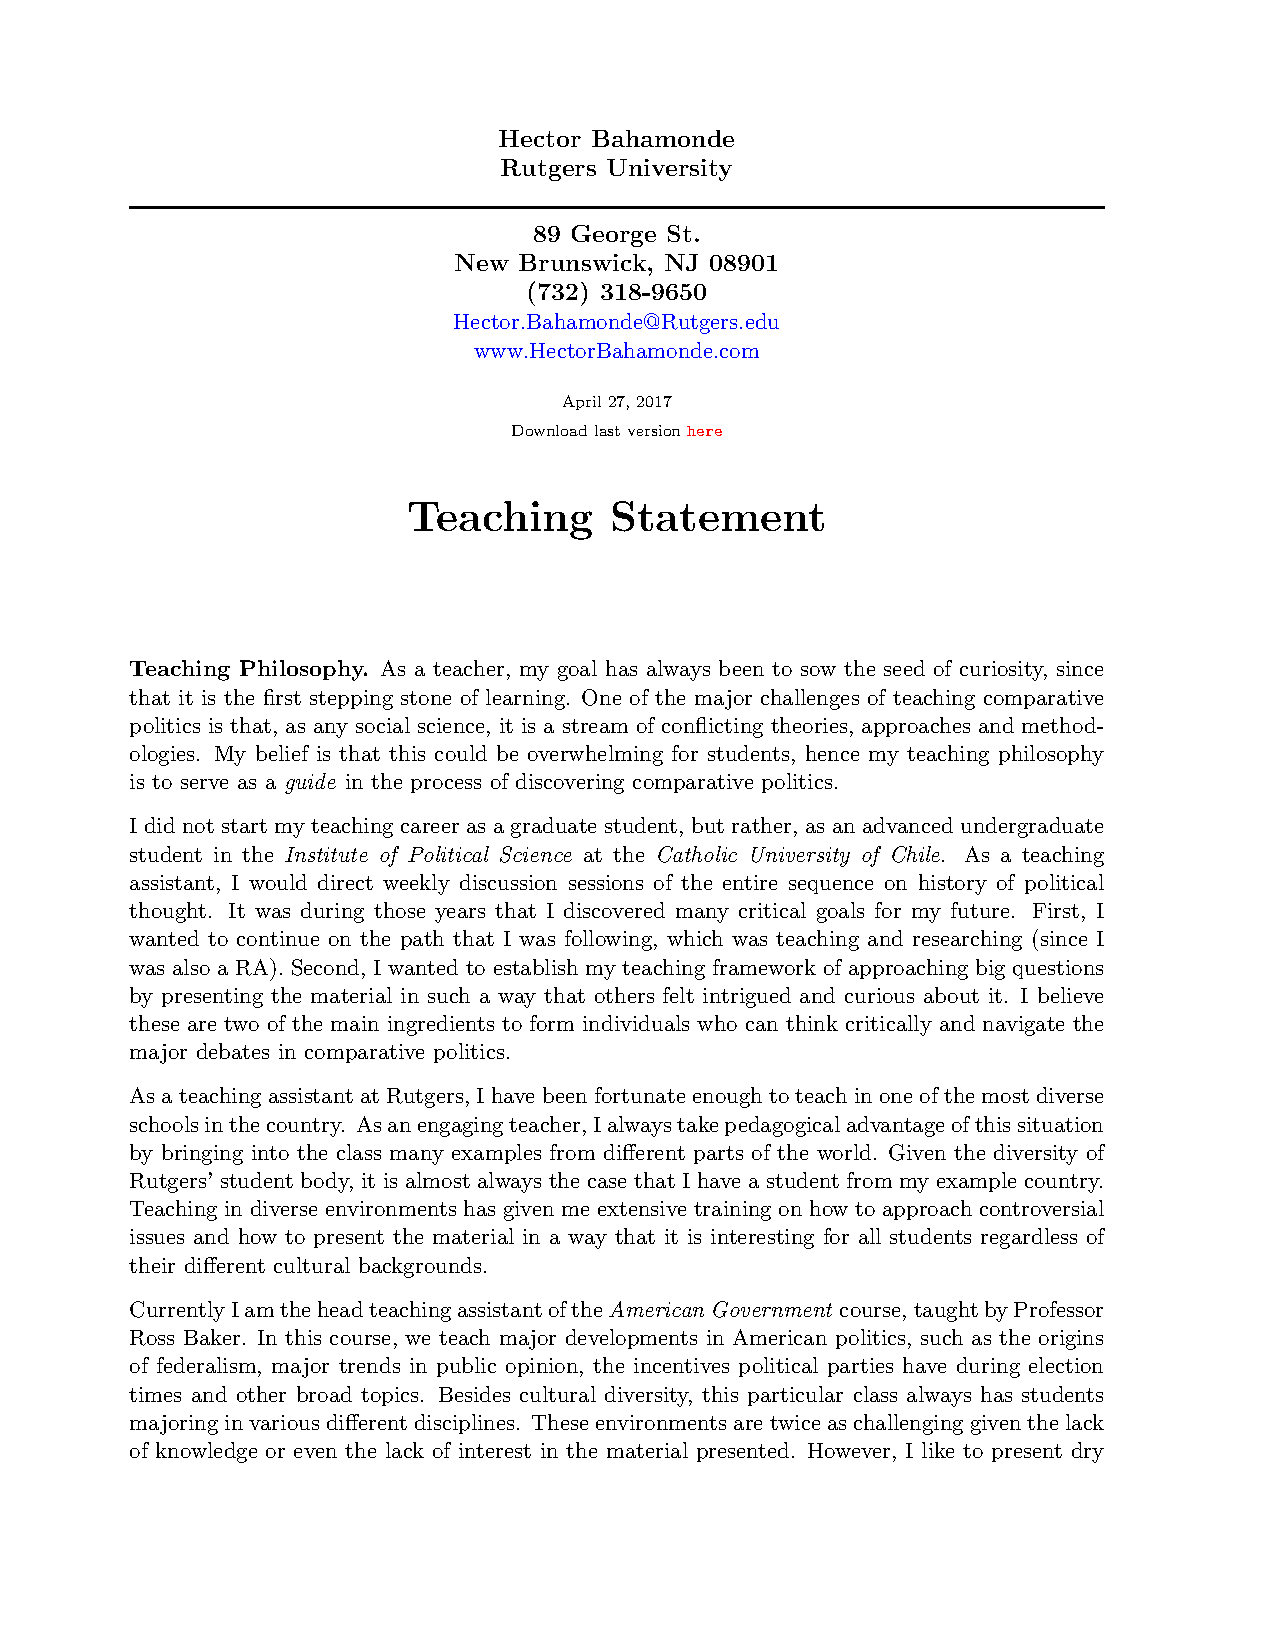
\includepdf[pages=-,addtotoc={1,section,1,Teaching Statement,Teaching Statement},pagecommand={\phantomsection{}{}}]{/Users/hectorbahamonde/Job_Market/Bahamonde_Teaching_Statement_LAC.pdf}


% Comparative UG
\includepdf[pages=-,addtotoc={1,section,1,Syllabus: Comparative Politics (UGrad),CPUgrad},
pagecommand={\phantomsection{}{}}]{/Users/hectorbahamonde/Teaching/Comparative_Politics_UGRAD/Bahamonde_Comparative_Politics_Syllabus_UGRAD.pdf}



% Lat. Am. Politics UG
\includepdf[pages=-,addtotoc={1,section,2,Syllabus: Latin American Politics (UGrad),LatAmPolUgrad},
pagecommand={\phantomsection{}{}}]{/Users/hectorbahamonde/Teaching/Latin_American_Politics_UGRAD/Bahamonde_Latin_American_Politics_Syllabus_UGRAD.pdf}

% Pol. Econ UG
\includepdf[pages=-,addtotoc={1,section,2,Syllabus: Introduction to Political Economy (UGrad),PolEconUgrad},
pagecommand={\phantomsection{}{}}]{/Users/hectorbahamonde/Teaching/Political-Economy-Intro-UGrad/Pol_Econ_Dev_Syllabus_UGRAD.pdf}

% Teaching Evaluations Fall 2017
\includepdf[pages=-,addtotoc={1,section,2,Most Recent Teaching Evaluations,TeachEvS2017},
pagecommand={\phantomsection{}{}}]{/Users/hectorbahamonde/Resources/Bahamonde_Most_Recent_Teaching_Evs.pdf}


\end{document}







